\documentclass[8pt]{beamer}

% ****************
% ***** INFO *****
% ****************
\usepackage[english]{babel}
\title[Boğazici University]{Shifting Rhetoric: The Rise of Pro-Nationalist Discourse in European Parliamentary Speeches (2009-2019)}

\author[Name Surname]{Andrea Cristiano, Furkan Kazanci} 
\institute[]{Boğazici University}
\newcommand{\currentyear}{\the\year} % \currentyear
\newcommand{\nextyear}{\the\numexpr\year+1\relax} % \nextyear
\date{\currentyear/\nextyear} % or \today

% *******************
% ***** PROJECT *****
% *******************
\definecolor{main}{HTML}{0000FF}
\setbeamercolor{structure}{fg=main}

% *****************
% ***** THEME *****
% *****************
\usetheme{Luebeck}
\usepackage{helvet}
\renewcommand{\familydefault}{\sfdefault}
\setbeamertemplate{frametitle continuation}{\gdef\beamer@frametitle{}}
\setbeamertemplate{footline}{}

% *****************
% ***** CODE *****
% *****************
\usepackage{listings}
\lstdefinestyle{java}{
    backgroundcolor=\color{white},
    basicstyle=\ttfamily\scriptsize,
    breaklines=true,
    commentstyle=\color{gray},
    keywordstyle=\color{blue},
    stringstyle=\color{magenta},
    identifierstyle=\color{black},
    numberstyle=\color{gray},
    language=Java
}
\lstdefinestyle{cpp}{
    backgroundcolor=\color{white},
    basicstyle=\ttfamily\scriptsize,
    breaklines=true,
    commentstyle=\color{gray},
    keywordstyle=\color{blue},
    stringstyle=\color{magenta},
    identifierstyle=\color{black},
    numberstyle=\color{gray},
    language=C++
}
\lstdefinestyle{py}{
    backgroundcolor=\color{white},
    basicstyle=\ttfamily\scriptsize,
    breaklines=true,
    commentstyle=\color{gray},
    keywordstyle=\color{blue},
    stringstyle=\color{magenta},
    language=Python
}
\lstdefinestyle{js}{
    backgroundcolor=\color{white},
    basicstyle=\ttfamily\scriptsize,
    breaklines=true,
    commentstyle=\color{gray},
    keywordstyle=\color{blue},
    stringstyle=\color{magenta},
    identifierstyle=\color{black},
    numberstyle=\color{gray},
    language=JavaScript,
    escapechar=@
}
\lstdefinestyle{sh}{
    basicstyle=\ttfamily\scriptsize,
    breaklines=true,
    commentstyle=\color{gray},
    keywordstyle=\color{blue},
    stringstyle=\color{magenta},
    identifierstyle=\color{black},
    numberstyle=\color{gray},
    language=bash
}

% **********************
% ***** ALGORITHMS *****
% **********************
\usepackage{algorithm}
\usepackage{algpseudocode}

% *****************
% ***** UTILS *****
% *****************
\usepackage{xcolor}

% ********************
% ***** DOCUMENT *****
% ********************
\begin{document}

% **********************
% ***** TITLEPAGE ******
% **********************
\begin{frame}{}
\vspace{\fill}



\vspace{\fill}

\Large
\color{main}
\inserttitle

\medskip

\large
\color{black}
\insertsubtitle

\vspace{\fill}

\footnotesize
\insertinstitute

\vspace{\fill}

\textbf{Author:} \insertauthor

\medskip

\insertdate

\vspace{\fill}
\end{frame}

% *****************
% ***** START *****
% *****************

\begin{frame}[allowframebreaks]{Introduction}
\small
\textbf{Key Points}: 
\begin{itemize}
    \item Post-WWII liberal-progressive policies emphasized economic cooperation and democratic values.
    \item Crises of 2008 (financial) and 2015 (refugee) fueled nationalist rhetoric.
    \item Nationalism challenges neoliberal values through sovereignty and identity narratives.
    \item Increasing relevance of nationalist rhetoric across political spectrums in Europe.
\end{itemize}

\textbf{Main Goals}:
\begin{itemize}
    \item Analyze the longitudinal trends in nationalist rhetoric in France, Hungary, and the UK.
    \item Investigate whether rhetoric evolved based on political affiliation and country.
    \item Assess tone shifts using sentiment analysis.
\end{itemize}

\end{frame}

\begin{frame}{Theoretical Framework}

\begin{itemize}
    \item \textbf{Core Concepts of Nationalism}:
    \begin{itemize}
        \item Ethnic Nationalism: Based on shared culture, language, and heritage.
        \item  Civic Nationalism: Focused on citizenship and equal rights.
        \item  Emotional Appeals: Used to "preserve" cultural and national. identity.
    \end{itemize}
    \item \textbf{Key Themes}:
    \begin{itemize}
        \item Migration: Integration challenges, border control.
        \item Cultural Hegemony: Preservation of Western-Christian values.
        \item  Ethnic Threat: Demographic and cultural shifts as "threats."
    \end{itemize}
\end{itemize}
    
\end{frame}

\begin{frame}{Related Work - Computational Approaches to Analyzing
Nationalist Discourse in European Parliaments}

\begin{enumerate}
    \item \textbf{Digital Parliamentary Datasets and Computational Social Sciences}
        \begin{itemize}
            \item Growing availability of structured datasets.
            \item  Enabling deeper comprehension of thematic shifts in political discourse.
        \end{itemize}
    \item \textbf{Thematic Word Sets for Political Analysis}

        \begin{itemize}
            \item Tailored word sets critical for extracting patterns from large datasets.
            \item  Relevant themes: Ethnic threat, migration, cultural hegemony.
        \end{itemize}
    \item \textbf{Key Studies Highlighting Computational Methods}
        \begin{itemize}
            \item \textbf{Navaretta and Hansen }(2020) \cite{navarretta2020identifying}
        
            \begin{itemize}
                \item Analysis of Danish Parliament speeches.
                \item Rhetorical and linguistic differences via NLP.
                \item Insights into party alignment and partisan framing.
            \end{itemize}
            \item \textbf{Søyland} (2020) \cite{soyland2020parliamentary}:
            \begin{itemize}
                \item Norwegian parliamentary debate analysis.
                \item  Topic modeling reveals patterns in electoral reforms and language evolution.
            \end{itemize}
        \end{itemize}

    \item \textbf{Transformative Potential of Computational Techniques}
    \begin{itemize}
        \item Bridging qualitative political analysis with large datasets.
        \item Advantages: Comparability, granularity, and scalability.
    \end{itemize}
\end{enumerate}

\textbf{Implications}:
\begin{itemize}
    \item Systematic categorization aids in assessing nationalist discourse.
    \item Computational approaches offer scalable, data-driven insights into political themes.
\end{itemize}

\end{frame}

\begin{frame}{Research questions}

\textbf{Research Questions}:

\begin{itemize}
    \item \textbf{RQ1}: How has the frequency of nationalist rhetoric evolved in parliamentary speeches (2009-2019)?
    \item \textbf{RQ2}: Has the tone of nationalist rhetoric become increasingly negative over time?
\end{itemize}

\textbf{Hypotheses}:

\begin{itemize}
    \item \textbf{H1}: Nationalist rhetoric has consistently increased over time.
    \item \textbf{H2}: The tone of nationalist rhetoric has become more negative, featuring ethnic threats and exclusionary narratives.
\end{itemize}
    
\end{frame}

\begin{frame}{Data}

    We used the  "\textbf{ParlEE plenary speeches data set: Annotated full-text of 21.6 million sentence-level plenary speeches of eight EU states}" \cite{sylvester2022parlee} dataset.

    Contains the full speeches from the legislative chambers of:  

    Austria, Belgium, France, Germany, Hungary, Ireland, Portugal and the United Kingdom, covering the \textbf{2009-2019} period.  

    
\end{frame}

\begin{frame}{Data - Preprocessing}

    \begin{columns}[T]
        \begin{column}{0.5\textwidth}
            The main preprocessing step was a \textbf{filtering} operation. We analyzed only those speeches containing some keywords related to the topic.

            Since the speeches in the dataset weren't translated in English, we generated a set of word for each of the involved languages. 

            
        \end{column}
        \begin{column}{0.5\textwidth}
            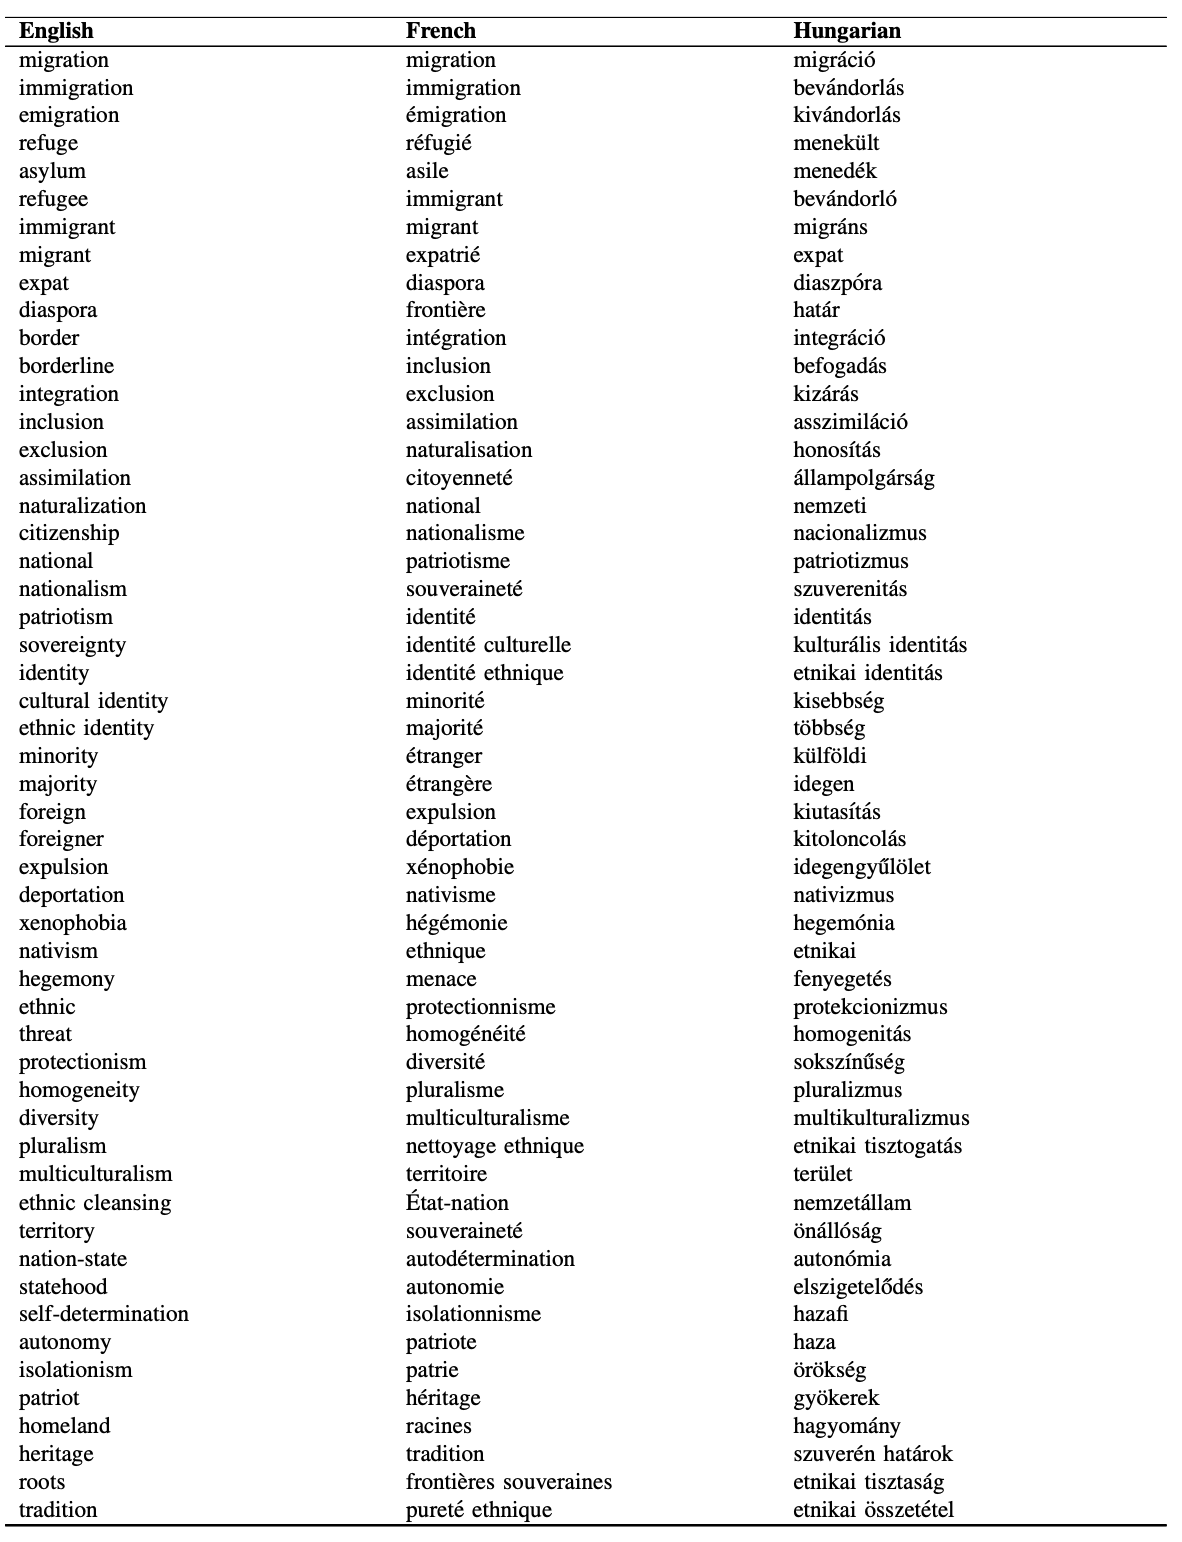
\includegraphics[width=\textwidth]{img/Dictionary.png}
        \end{column}
    \end{columns}
    
\end{frame}

\begin{frame}{Methodology}
    We used Sentiment analysis to analyze the content of the speeches.
    \begin{itemize}
        \item \textbf{Definition}: Sentiment analysis is a Natural Language Processing (NLP) technique to evaluate and classify text as positive, negative, or neutral.
        \item \textbf{Objective}: Analyze the sentiment polarity of parliamentary speeches to detect trends in political discourse.
        \item \textbf{Methodology}:
        \begin{itemize}
            \item Lexicon-based analysis using the \texttt{TextBlob} library.
            \item Focused on detecting polarization in the discourse.
        \end{itemize}
        \item \textbf{Visualization}: Sentiment trends over time and party-level sentiment analysis for comparative insights.
    \end{itemize}

    \begin{columns}[T]
        \begin{column}{0.5\textwidth}
            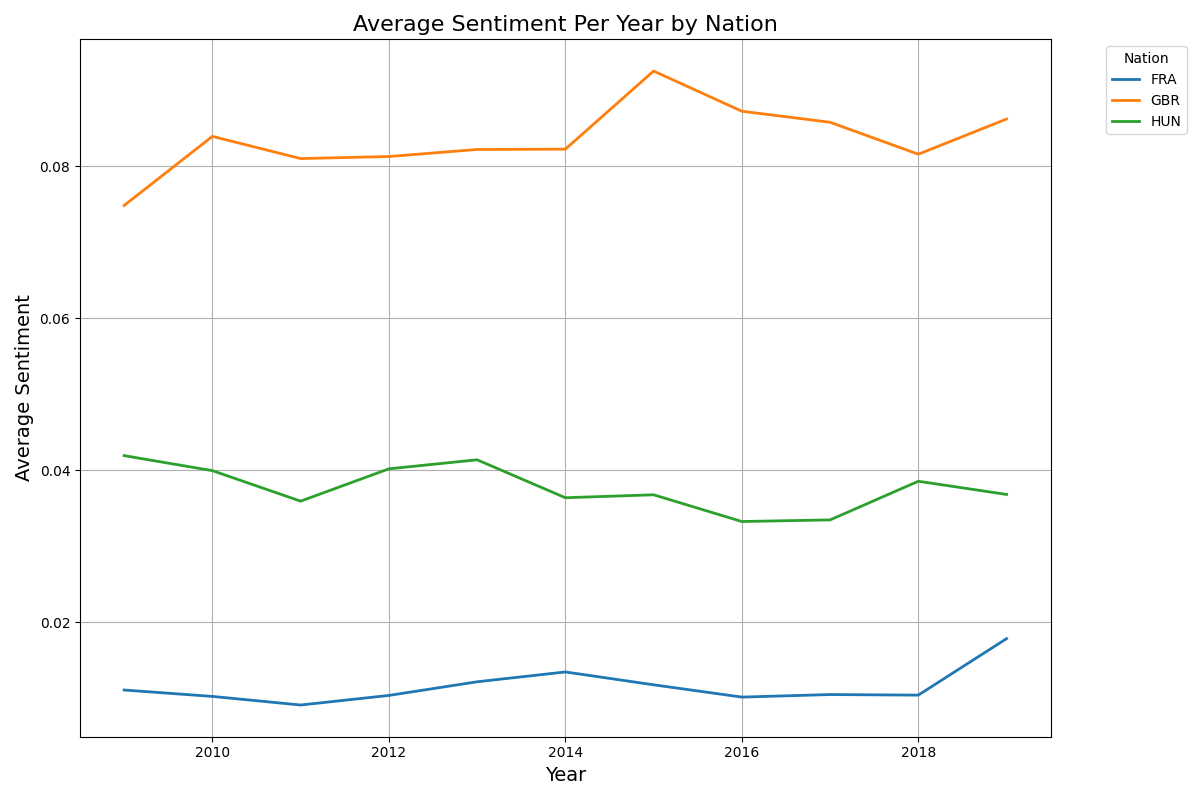
\includegraphics[width=\textwidth]{img/average_sentiment_per_year.png}
        \end{column}
        \begin{column}{0.5\textwidth}
            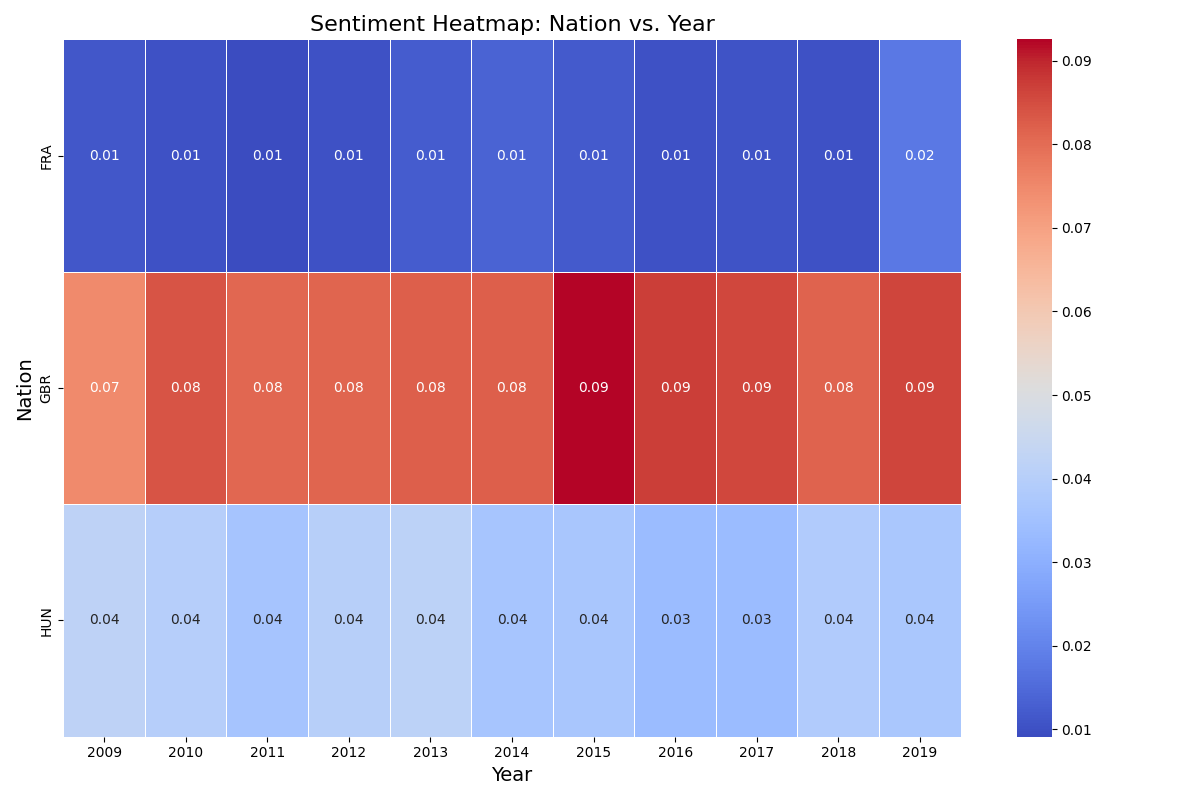
\includegraphics[width=\textwidth]{img/sentiment_heatmap.png}
        \end{column}
    \end{columns}
\end{frame}

\begin{frame}{Methodology}

\begin{columns}[T]
    \begin{column}{0.5\textwidth}
    
        Observing the Datapoints and average sentiment merics by themselves can lead to misinterpretation of the data.
        
        Thus there is the need to combine the two to get a metric which gives a clearer picture of the most influential parties in the discourse.
    \end{column}
    \begin{column}{0.5\textwidth}
        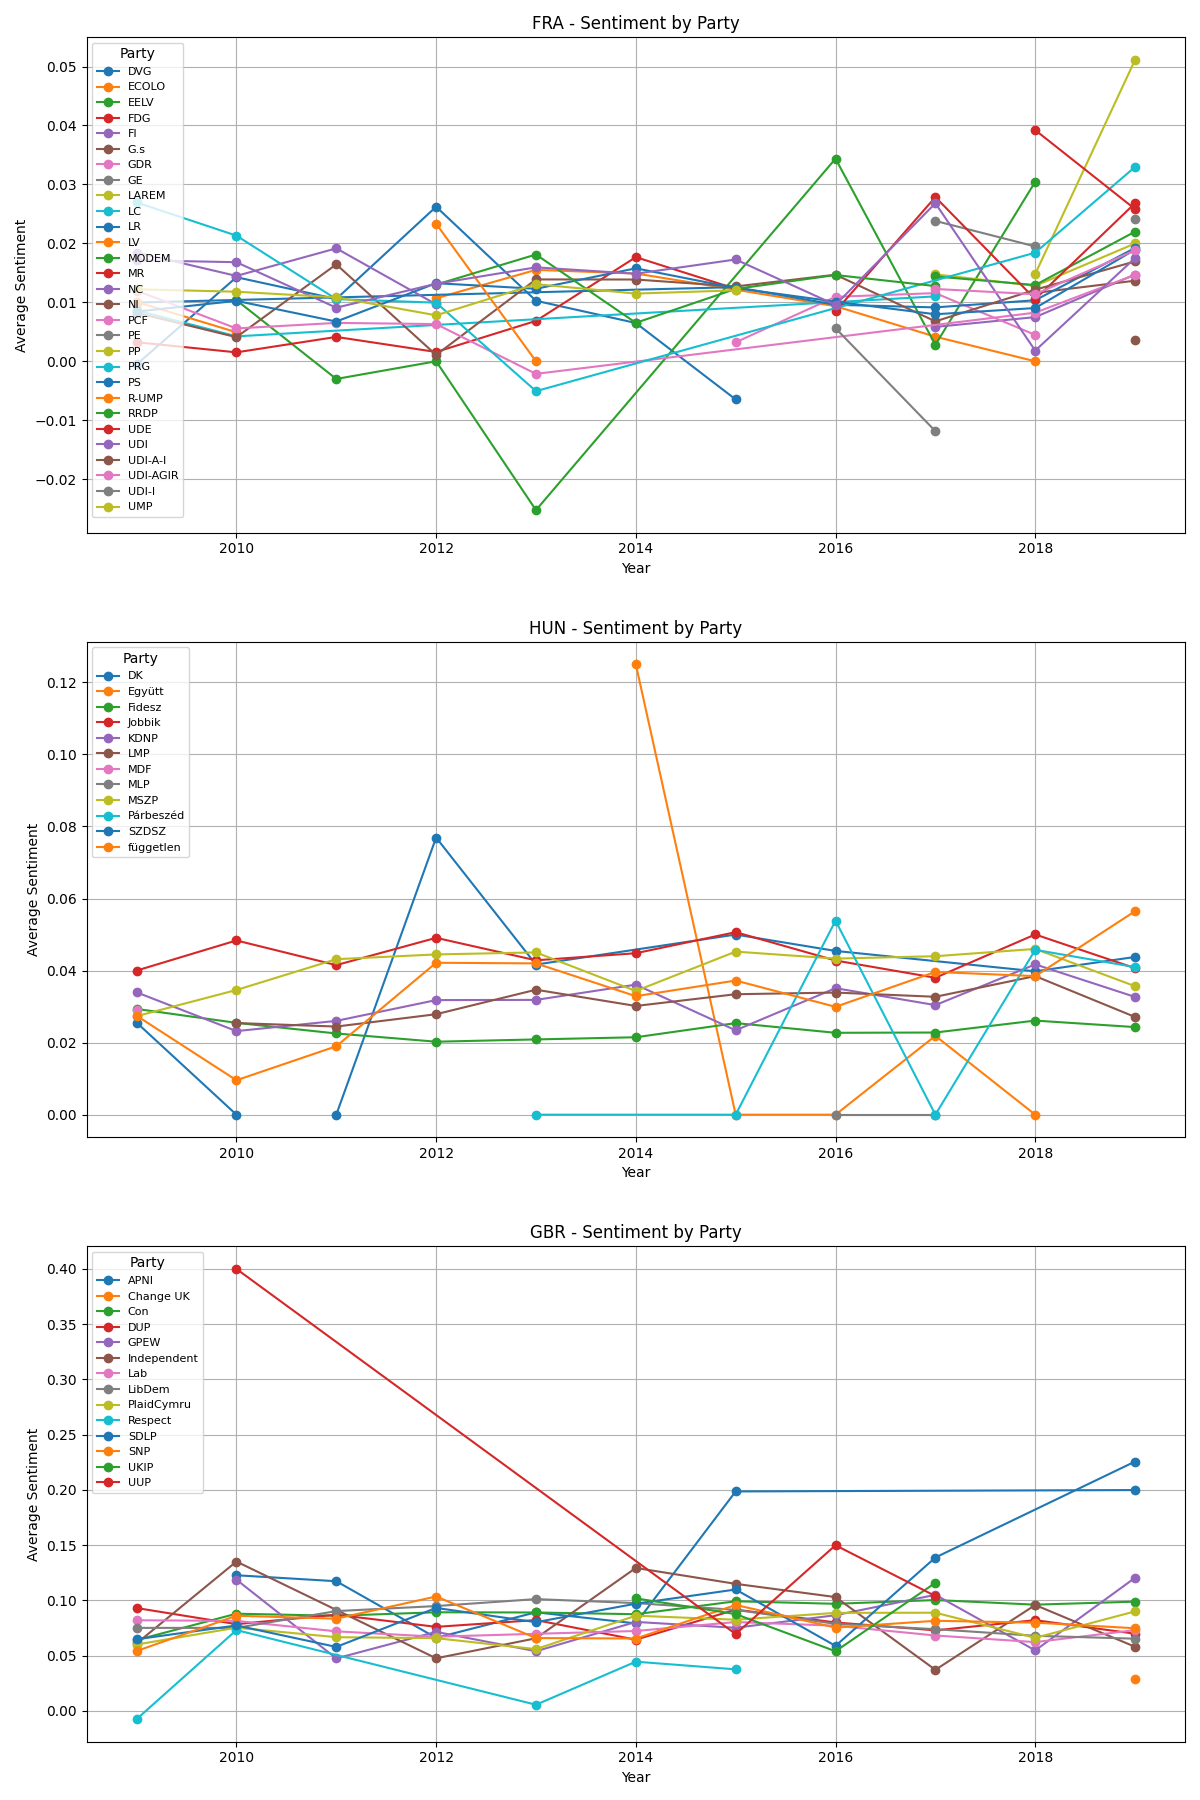
\includegraphics[width=\textwidth]{img/sentiment_by_party_3_rows.png}
    \end{column}
\end{columns}

    
\end{frame}

\begin{frame}{Results}
    \begin{columns}[T]
    \begin{column}{0.5\textwidth}
        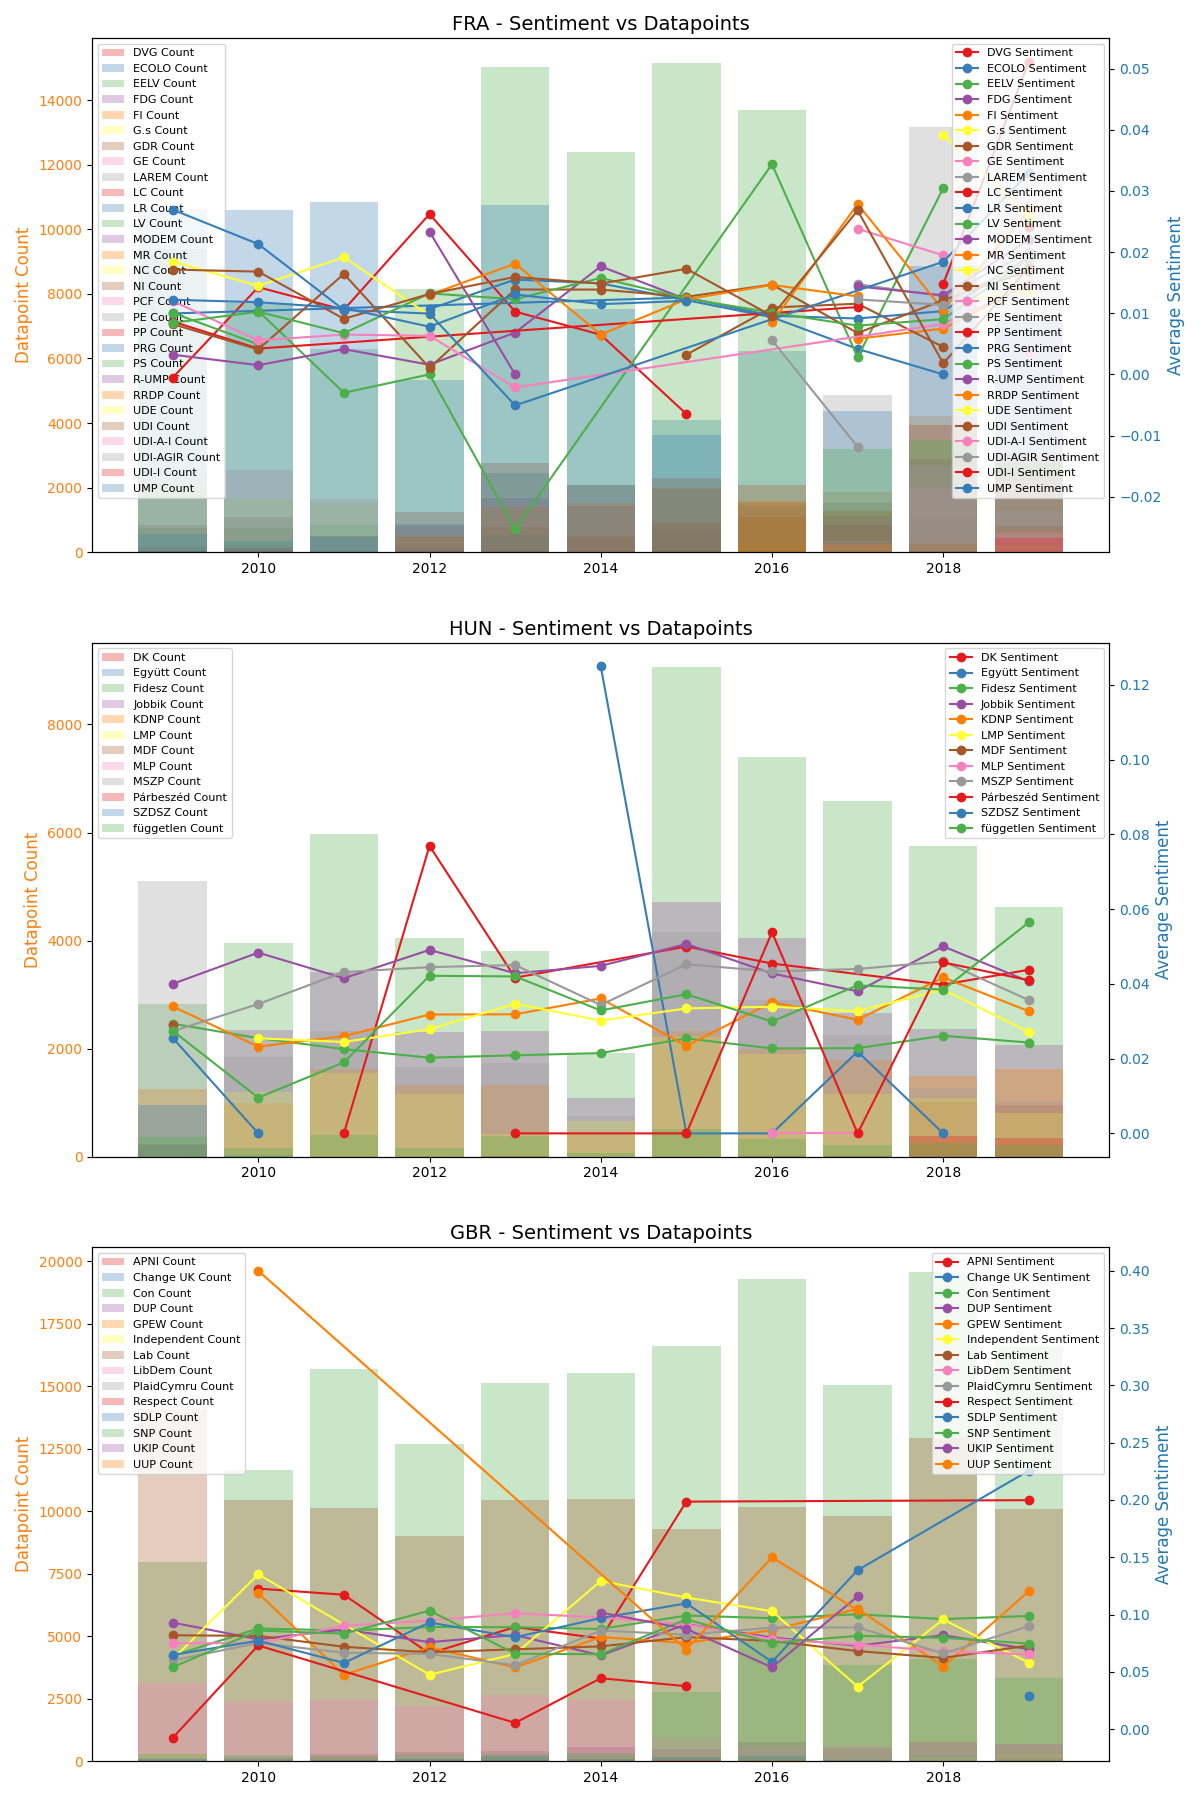
\includegraphics[width=\textwidth]{img/sentiment_and_datapoints_3_rows.png}
    \end{column}
    \begin{column}{0.5\textwidth}
        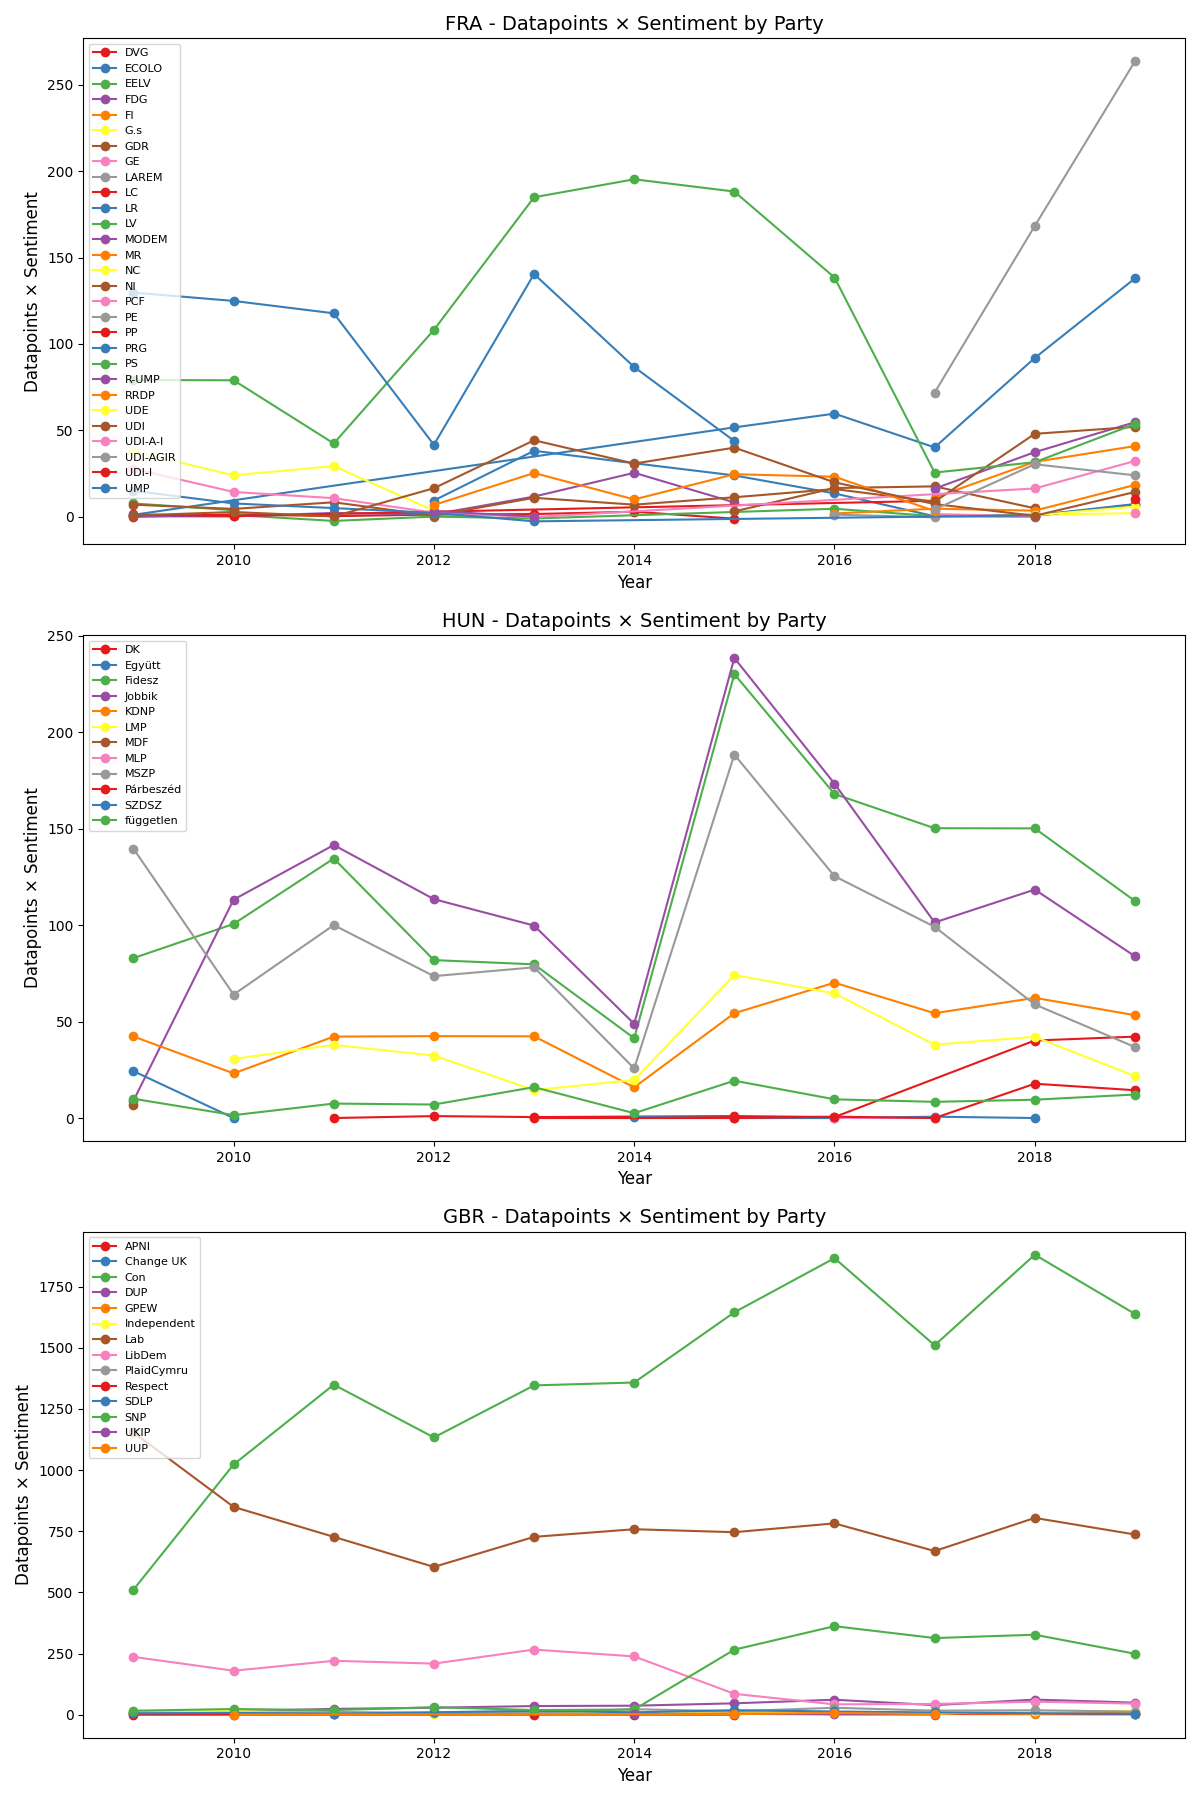
\includegraphics[width=\textwidth]{img/datapoints_times_sentiment_3_rows.png}
    \end{column}
\end{columns}
\end{frame}


\begin{frame}{Results Overview (H1)}
    \begin{columns}[T] % Align columns at the top
        \begin{column}{0.5\textwidth} % Left column with text
        \textbf{Findings}:
            \begin{itemize}
                \item \textbf{Hungary}: Spike in nationalist
                rhetoric in 2015 due to refugee
                crisis.
                \item \textbf{France}: Gradual increase, peaking
                in 2013 and 2018.
                \item  \textbf{UK}: Steady increase, notable peaks
                in 2016 (Brexit).
                
            \end{itemize}

        \textbf{Observations}:
        \begin{itemize}
            \item Contextual events (e.g., crises)
            drive discourse intensity.
            \item  Party-level dynamics crucial for
            understanding trends.
        \end{itemize}
        \end{column}
        \begin{column}{0.5\textwidth} % Right column with image
            \centering
            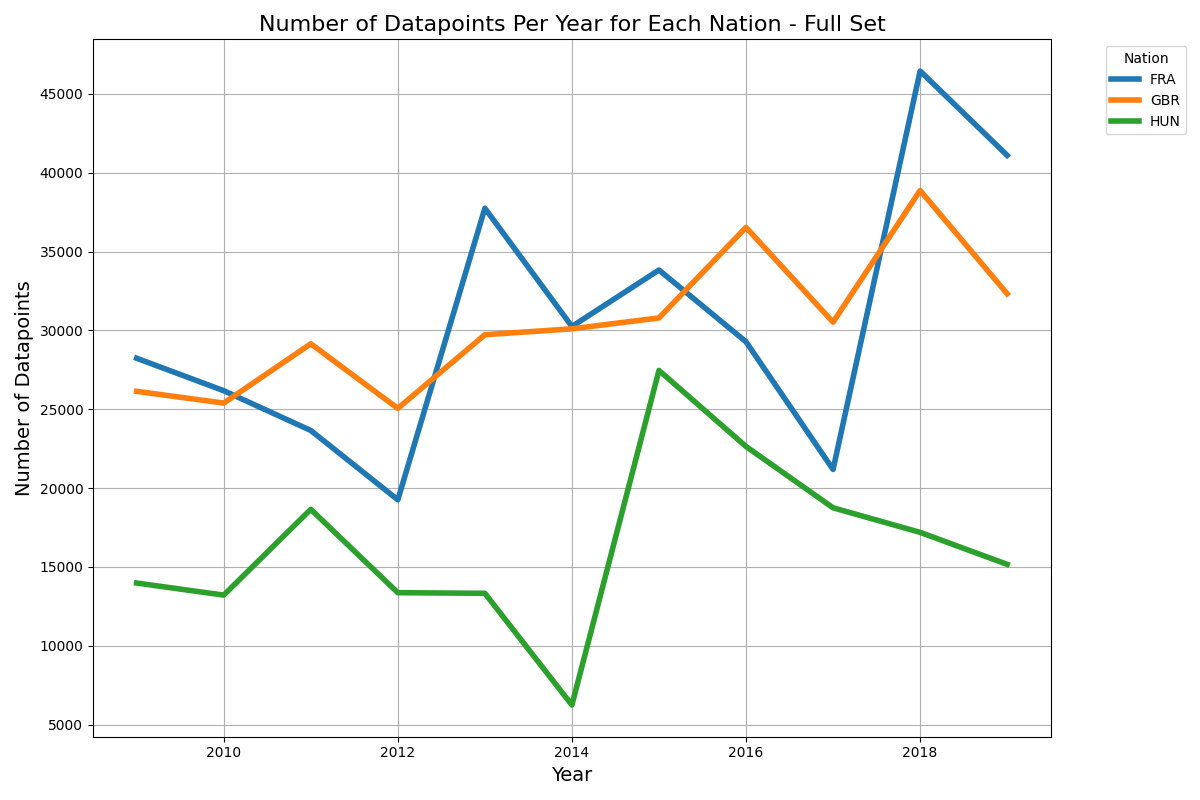
\includegraphics[width=\textwidth]{img/topicdatapoints_per_year.png}
            
        \end{column}
    \end{columns}

    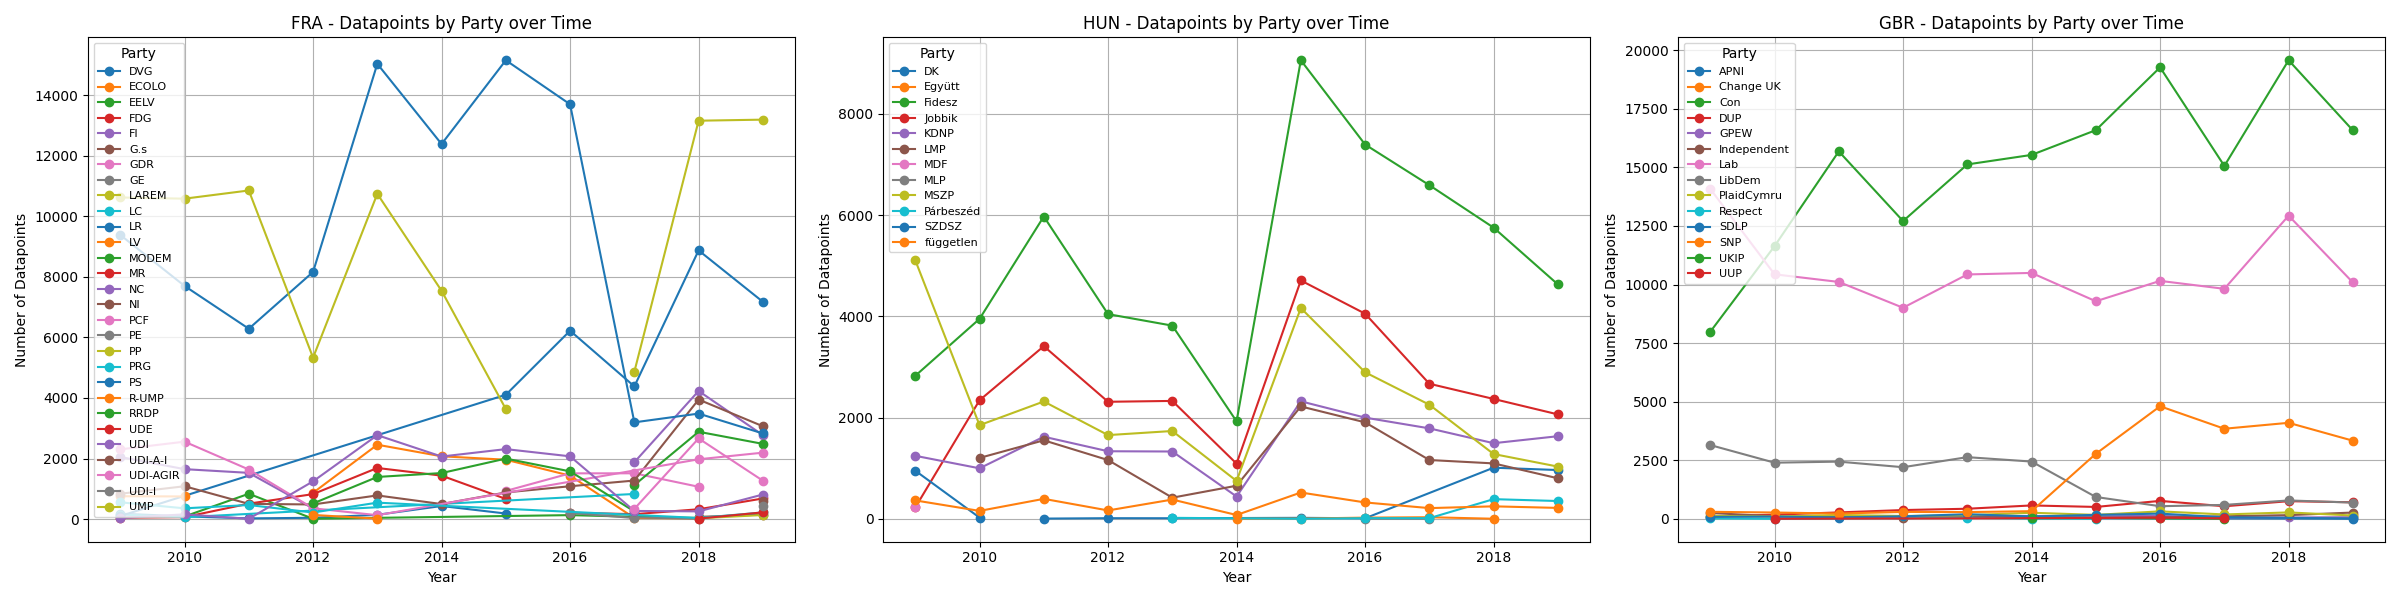
\includegraphics[width=\textwidth]{img/datapoints_by_party_and_year_3_columns.png}
\end{frame}

\begin{frame}{Results Overview (H2)}
        \begin{columns}[T] % Align columns at the top
            \begin{column}{0.5\textwidth} % Left column with text
            \textbf{Sentiment Analysis}:
    \begin{itemize}
        \item  \textbf{UK}: More nationalist tone overall.
        \item  \textbf{Hungary}: Neutral-leaning with spikes of nationalism post-2015.
        \item  \textbf{France}: Neutral tone, with increasing nationalist rhetoric in recent years.
    \end{itemize}
    
    \textbf{Key Observations}:
    \begin{itemize}
        \item Tone shifts reflect political and cultural crises (e.g., terror attacks in France).
        \item  Right-wing parties consistently use more nationalist rhetoric.
    ● Fig.. Combined metrics datapoints x sentiment analysis
    \end{itemize}
            \end{column}
            \begin{column}{0.5\textwidth} % Right column with image
                \centering
                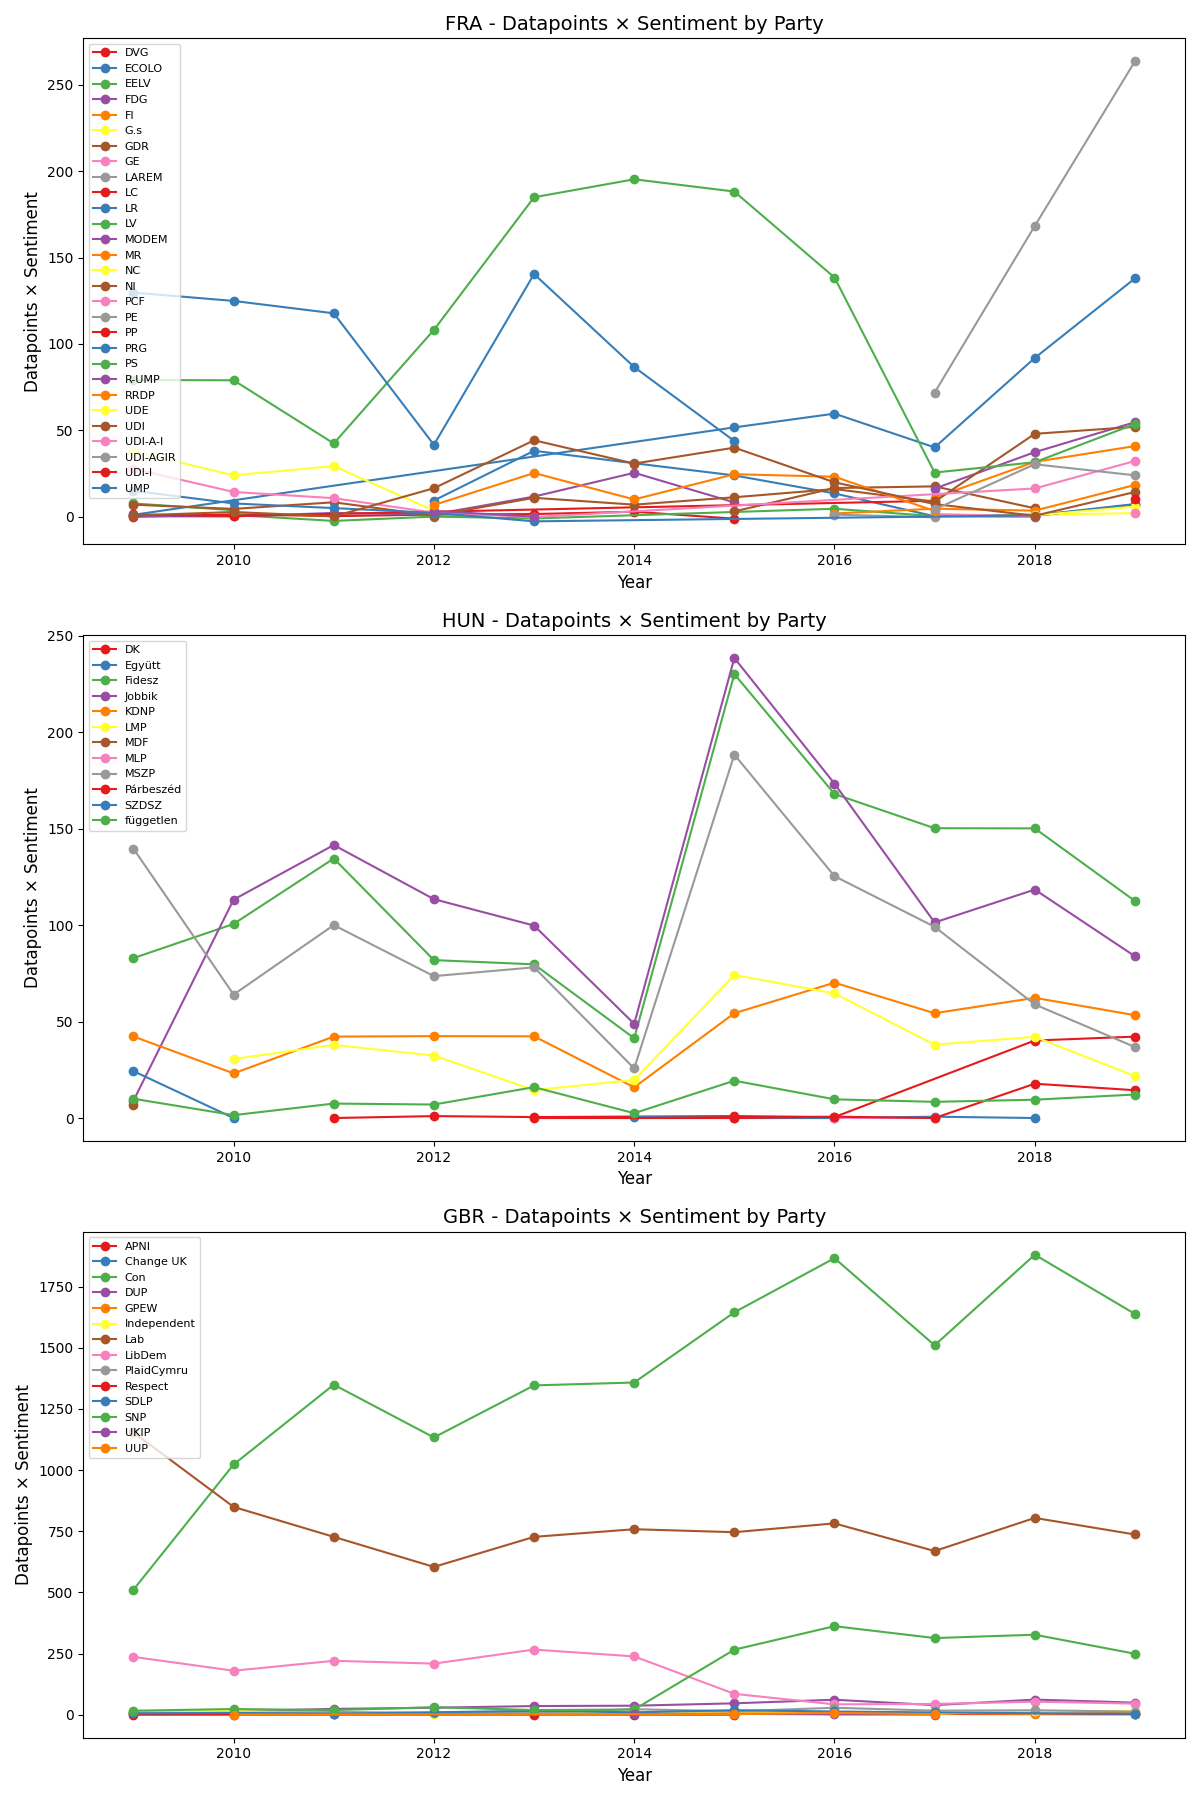
\includegraphics[width=\textwidth]{img/datapoints_times_sentiment_3_rows.png}
                
            \end{column}
        \end{columns}
\end{frame}

\begin{frame}{France}
    \begin{columns}
        
    
    \begin{column}{0.5\textwidth} % Right column with image
        \centering
        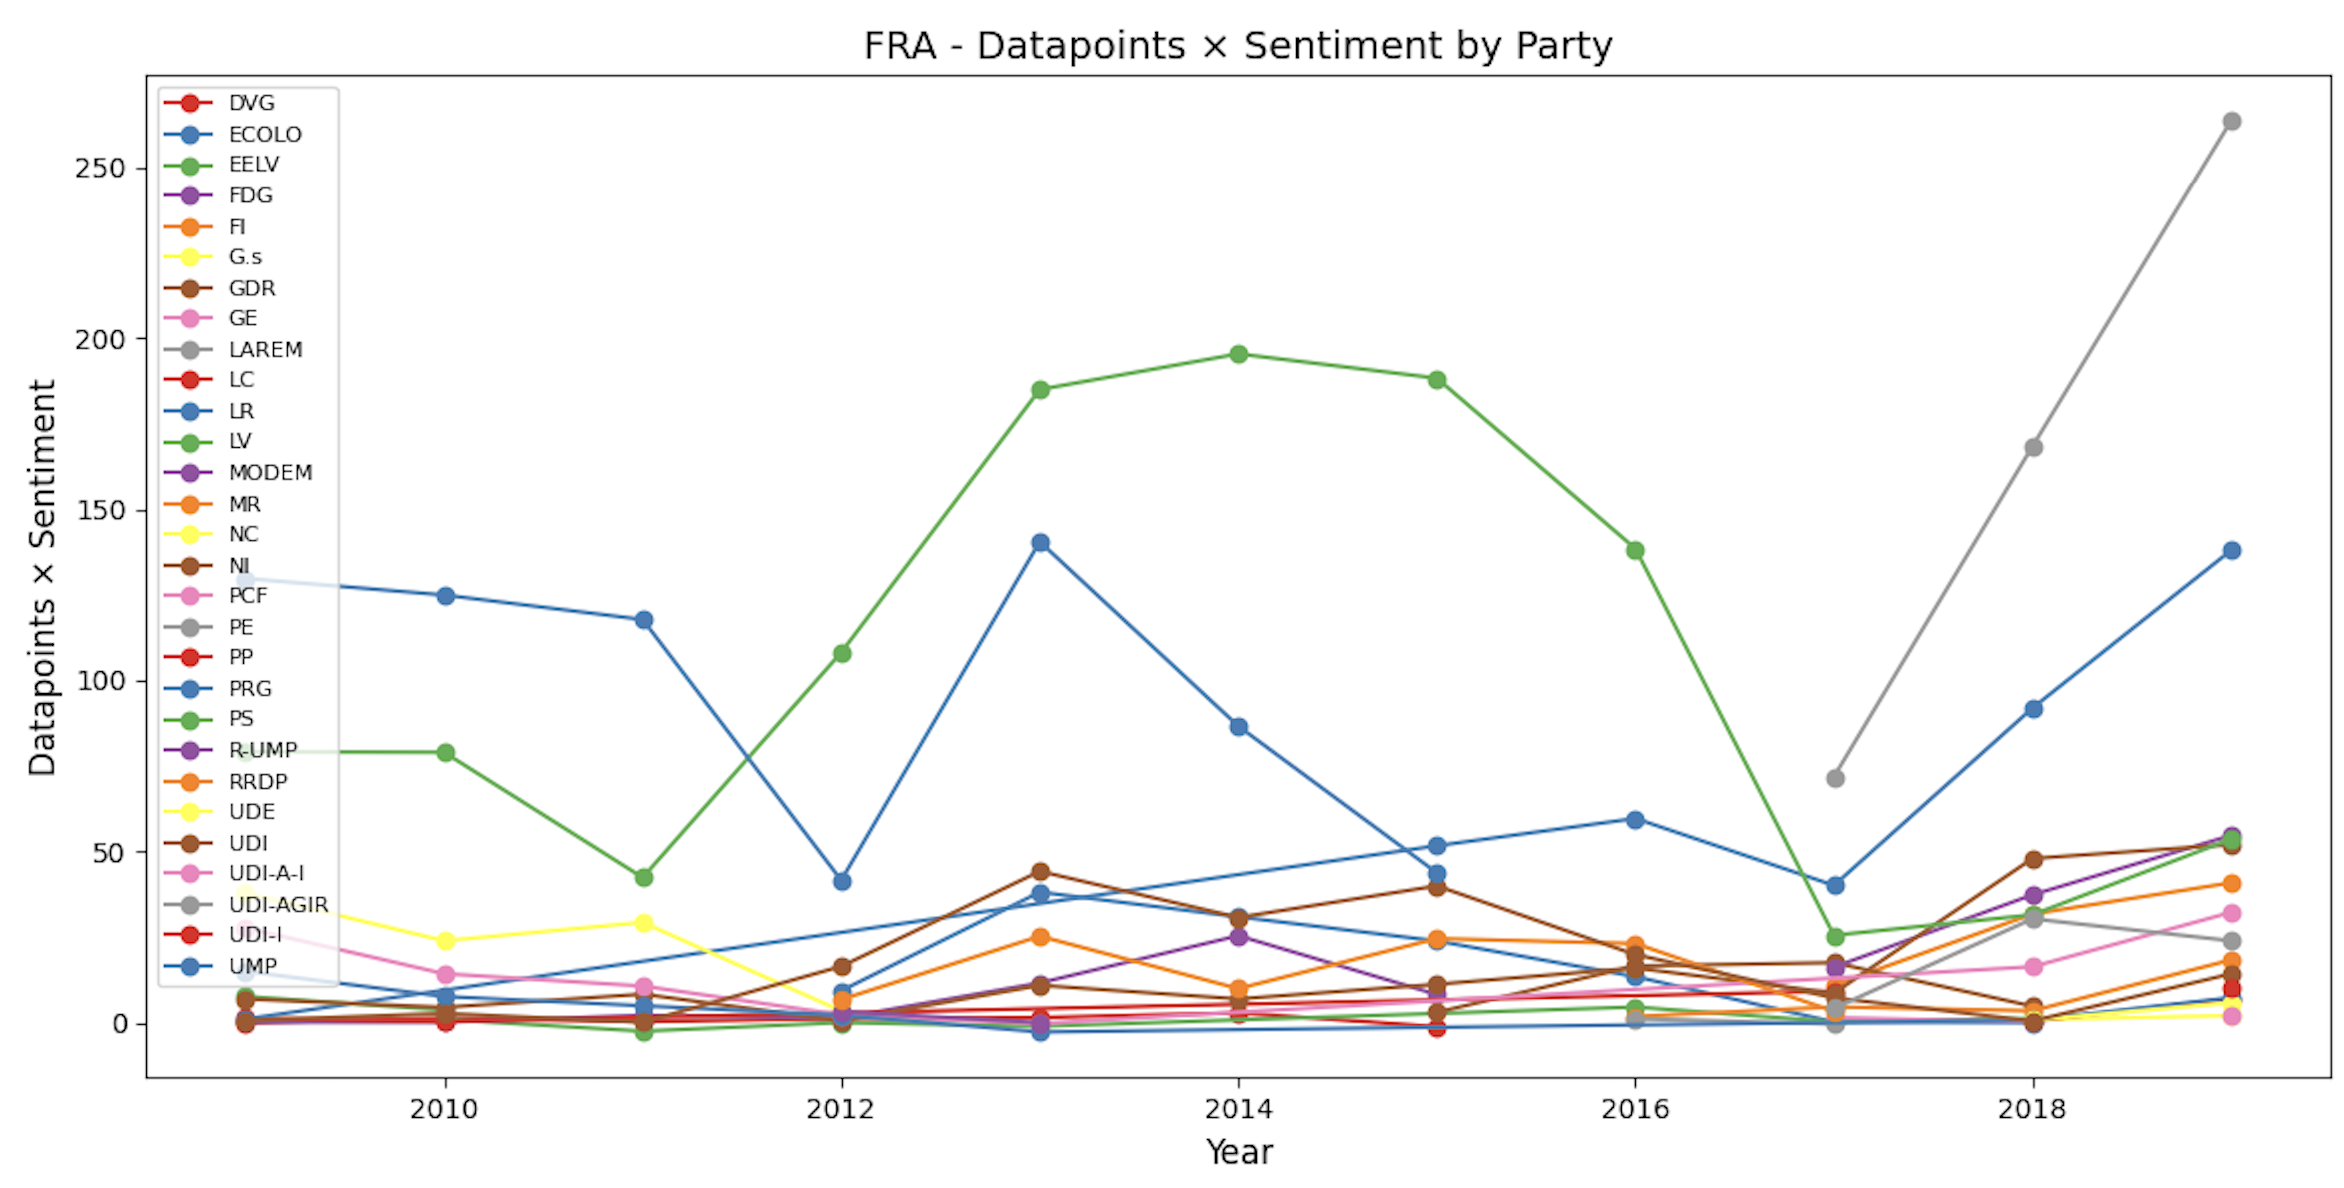
\includegraphics[width=\textwidth]{img/FRA.png}
        
    \end{column}

    \begin{column}{0.5\textwidth} % Right column with image
        \centering
        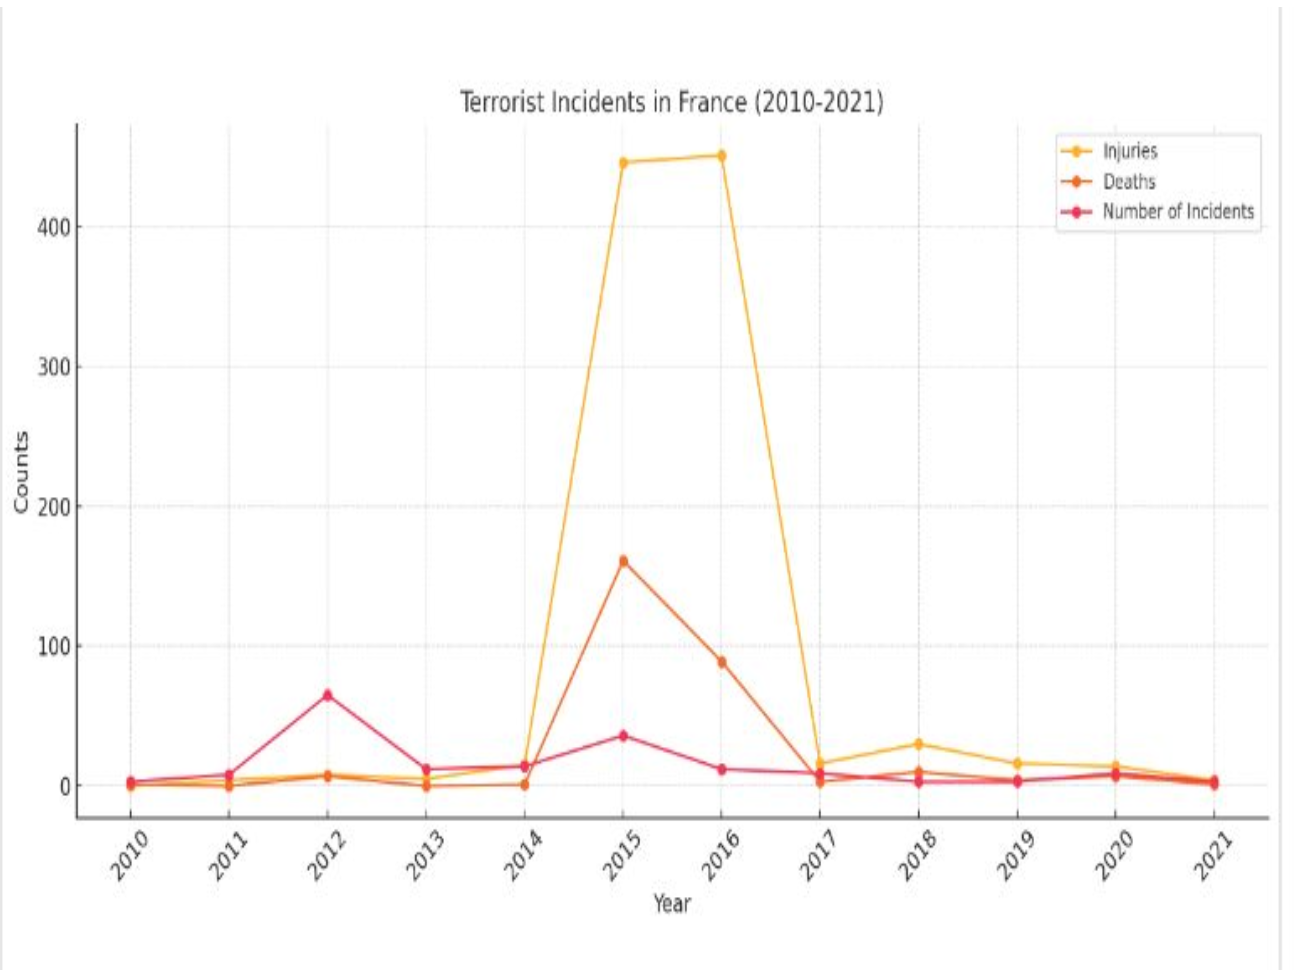
\includegraphics[width=\textwidth]{img/terrorism.png}
        
    \end{column}
    \end{columns}
\end{frame}

\begin{frame}{Hungary}

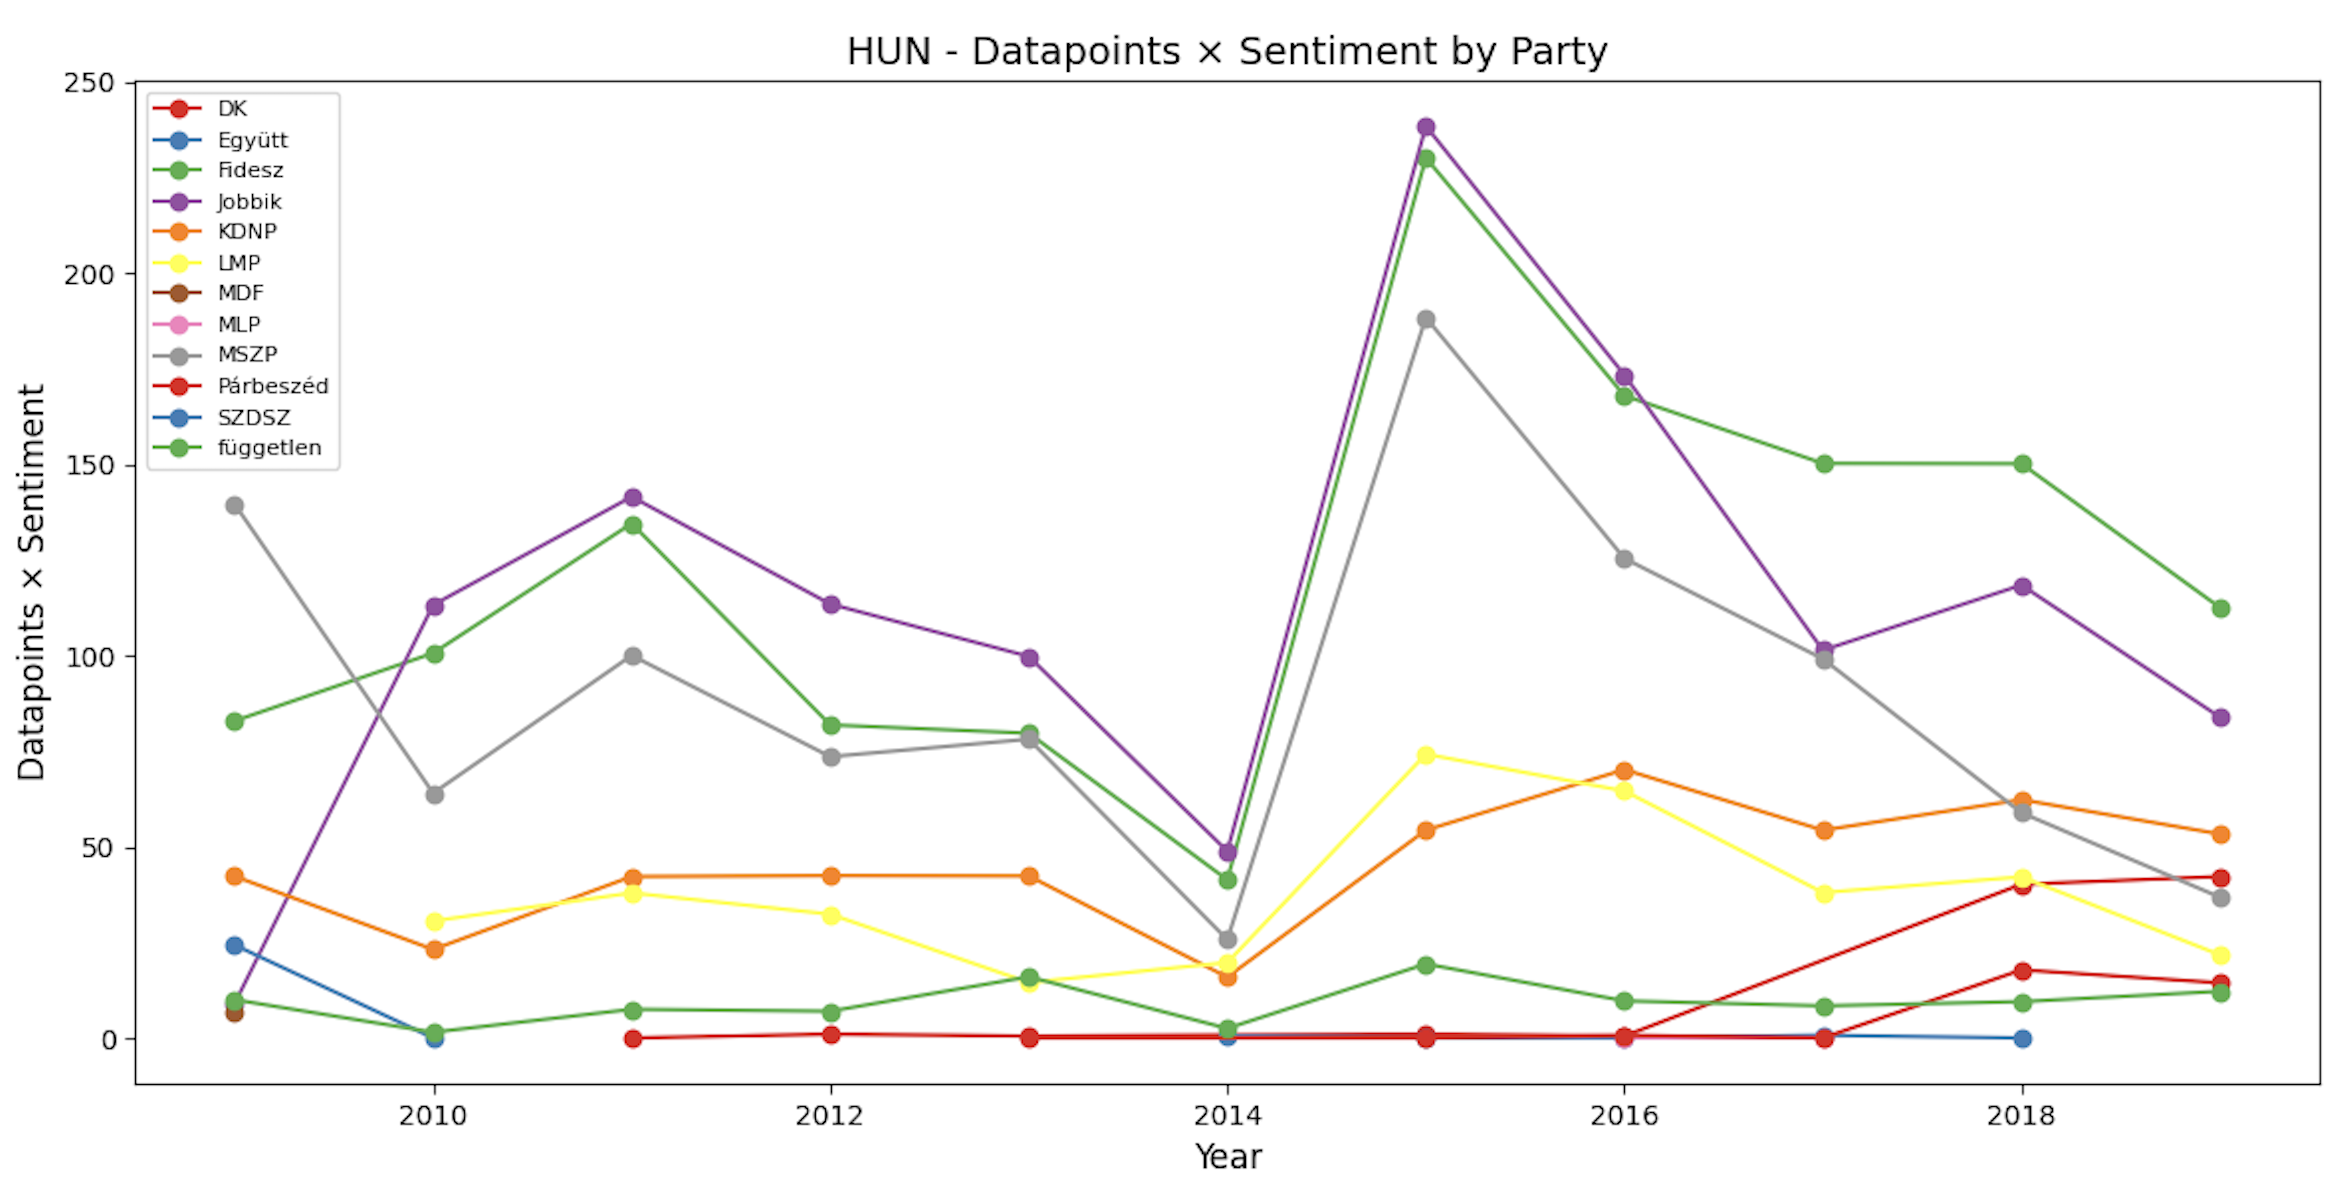
\includegraphics[width=\textwidth]{img/HUN.png}
    
\end{frame}

\begin{frame}{}
    \includegraphics[width=\textwidth]{img/refugees.png}
\end{frame}

\begin{frame}{Great Britain}
    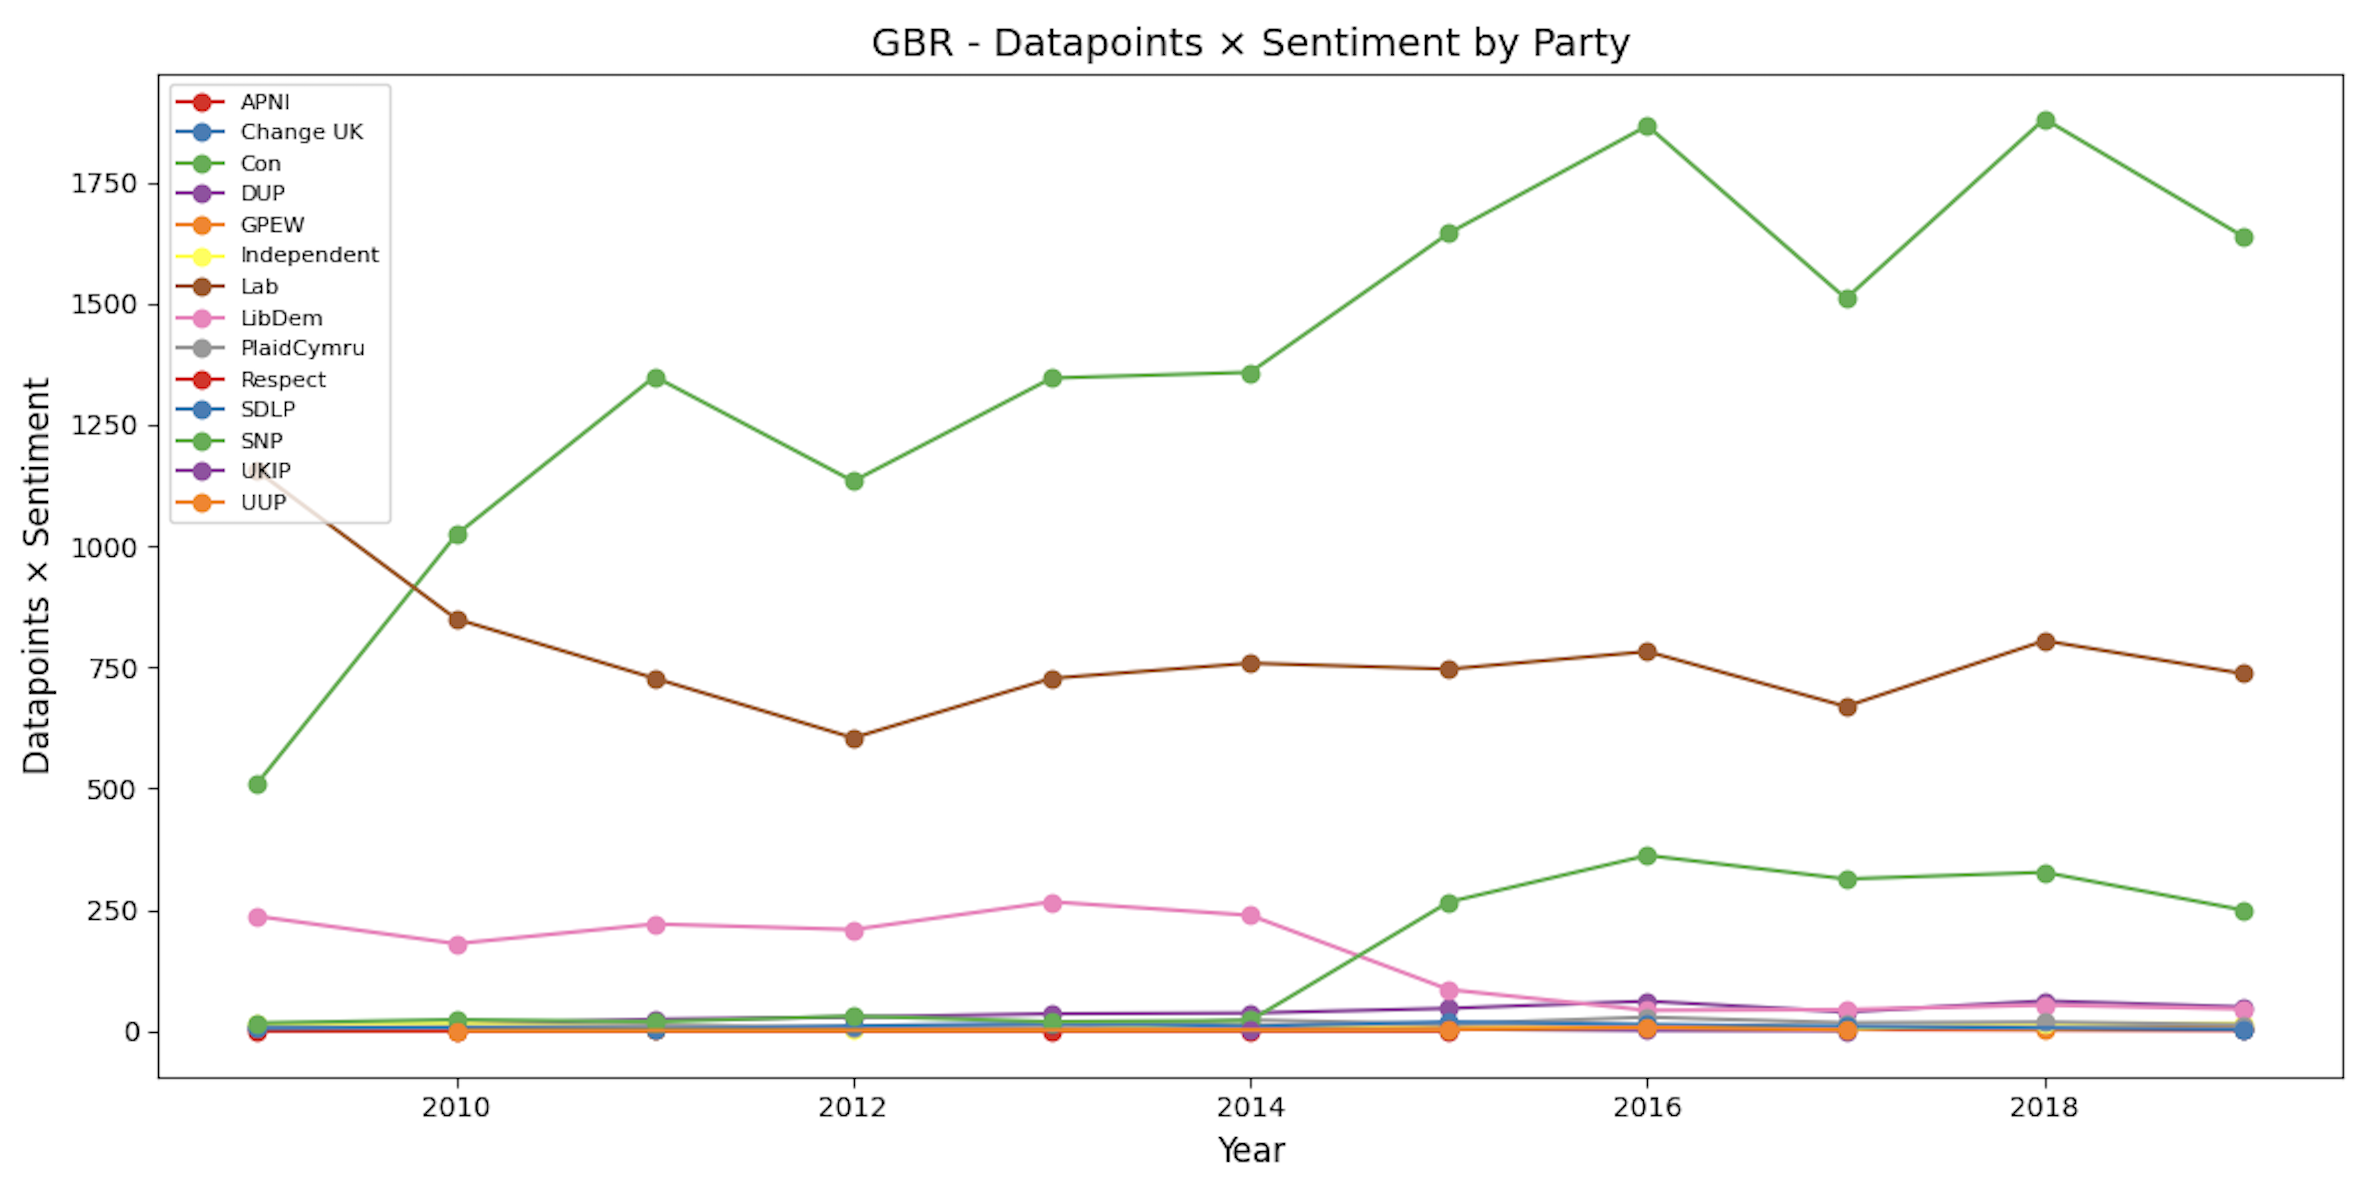
\includegraphics[width=\textwidth]{img/GBR.png}
\end{frame}

\begin{frame}{Discussion}
    \textbf{Main insights}:
    \begin{itemize}
        \item Contextual crises (e.g., refugee and financial) significantly shaped rhetoric.
\item  Hungarian and French cases partially support H1 and H2.
\item  UK case strongly supports both hypotheses.
    \end{itemize}
     \textbf{Trends}:
     \begin{itemize}
         \item Increasing use of exclusionary narratives across all parties.
\item  Sentiment stability masks deeper party-specific trends.
     \end{itemize}
\end{frame}

\begin{frame}{Limitations and Future Research}

    \textbf{Limitations}:
        \begin{itemize}
            \item Focus on three countries limits broader applicability.
\item  Data volume variations between parties and years.
        \end{itemize}
        \textbf{Future Directions}:
        \begin{itemize}
            \item Expand study to include more European countries.
            \item  Explore additional crises and their impact on discourse.
        \end{itemize}
    
\end{frame}

\begin{frame}{Conclusion}
\textbf{Key Takeaways}:
\begin{itemize}
    \item Nationalist rhetoric is rising across Europe, driven by crises and socio-political changes.
\item  Computational methods provide nuanced insights into political discourse.
\item  Nationalism’s tone and frequency are shaped by both global and local factors.
\end{itemize}
\textbf{Final Thought}:
\begin{itemize}
    \item Understanding political rhetoric is key to navigating future socio-political challenges.
\end{itemize}
    
\end{frame}

\begin{frame}{}
    Thanks for the attention!
\end{frame}


% ************************
% ***** BIBLIOGRAPHY *****
% ************************
\bibliographystyle{plain}
\bibliography{bib/references}
% ***************
% ***** END *****
% ***************

\end{document}